%
% DS 5110 (Blue Team) Project Proposal
%
\documentclass[12pt]{article}

%
% Packages
%
\usepackage{amsmath}
\usepackage{enumerate}
\usepackage[utf8]{inputenc}

\RequirePackage{graphics}

\usepackage{graphicx}
\graphicspath{ {imgs/} }

%
% Document Settings
%
\setlength{\parskip}{1pc}
\setlength{\parindent}{0pt}
\setlength{\topmargin}{-3pc}
\setlength{\textheight}{9.5in}
\setlength{\oddsidemargin}{0pc}
\setlength{\evensidemargin}{0pc}
\setlength{\textwidth}{6.5in}

\title{Property Assessment Visualization for the City of Boston}
\author{Tyler Brown, Sicheng Hao, Nischal Mahaveer Chand, Sumedh Sankhe}
\date{ }


% START DOCUMENT
\begin{document}

\maketitle

\section*{Summary}

When we put ourselves in the shoes of potential Greater Boston area
homebuyers, we find they have many informational resources available
to them. As a homebuyer, their major sources of information are the
websites Zillow \cite{ZillowRe12:online} and Trulia
\cite{TruliaRe98:online}. These resources provide information such as
home location, price, amenties, and types. Trulia differentiates itself
by providing a ``Local Scoop'', giving the homebuyer maps of crime, school
location, and the relative distribution of home prices in Greater
Boston. However, neither of these websites provide information about how
neighborhoods are changing over time.

Homebuyers want to better understand their potentially new communities.
It's helpful to know if your neighbors have been regularly developing
and maintaining their properties. A homebuyer would also like to know
whether a neighborhood has been experiencing various levels of turnover.
Our group is focusing on the problem new Greater Boston area home buyers
face when they want an intuitive way to understand changes within their
potential neighborhoods over time.

The City of Boston provides an open data platform, Analyze Boston, 
containing information related to our lives in the city. Property 
assessment data from 2014-2017 is one of the resources available on their
 open data platform. Included in the property assessment data is 
``property, or parcel, ownership together with information about value, 
which ensures fair assessment of Boston taxable and non-taxable property 
of all types and classifications'' \cite{Property49:online}. Our team 
has aggregated each available year to create a time series dataset of 
Property Assessments in Boston. This aggregated dataset allows us to 
provide unique insights into property valuations and ownership strategies.

\section*{Proposed Plan of Research}

The dataset we have right now is separated according to year in different
files. We will start by merging the data into a single file and completing
the necessary cleaning and data wrangling steps. We will then build a 
web application which provides the user with a helpful dashboard. This
dashboard will include a selection bar for their home preferences, and
a way to select which changes in the neighboorhood they want to
explore such as assessment changes or remodel status. We plan to improve
exploration of neighborhood changes by applying a clustering model to see
if patterns exists. The dashboard will also include an interactive map to
help users visualize those changes. 

\section*{Preliminary Results}

Our preliminary results include a data audit and descriptive findings.
The data audit found trouble spots in our data such as missing values or
incomplete values for coordinates as well as a small number of duplicate
values for the given primary keys. The descriptive findings generated
possible directions for our research question such as changes in 
property valuations, dominant ownership strategies for owners 
controlling a higher percentage of Boston property, and changes in
property valuations for various land usage types.

\subsection*{Data Audit Findings}

The major data audit findings are (1) the given primary keys, $PID$, are 
not unique for 0.3\% because they are mapped to multiple geographic 
coordinate pairs, (2) about 22\% of geographic coordinates are either 
missing or unusable, (3) about 10\% of property parcels, identified with
$PID$ do not pay taxes. Of that 10\%, we can explain about 49\% of this 
variation due to tax-exempt land use status. The remaining 51\% is 
associated with the "Condominium main" land usage type. It's unclear why 
there are zero taxes associated with this land usage type without 
contacting the city of Boston. This anomaly effects about 5\% of the 
total data.

\subsection*{Descriptive Findings}
Preliminary relationships found within the data are (1) residential 
condominium units appear to have the lowest proportion of value but 
previously we saw they had the second-highest proportion of gross tax,
(2) residential family and residential land appears to have gained the 
most value from 2014-2017, (3) the most significant gains in property
assessment from 2014-2017 have been made land used for commerical and
commerical condominium properties, (4) those who are further away from 
the financial district appear to be generally paying a lower proportion 
of taxes, and (5) larger real estate developers appear to choose one
of two distinct strategies that involve either paying higher taxes with
less property or lower taxes with more property. The figure below shows
how location might effect changes in property assessments from 2014-2017.

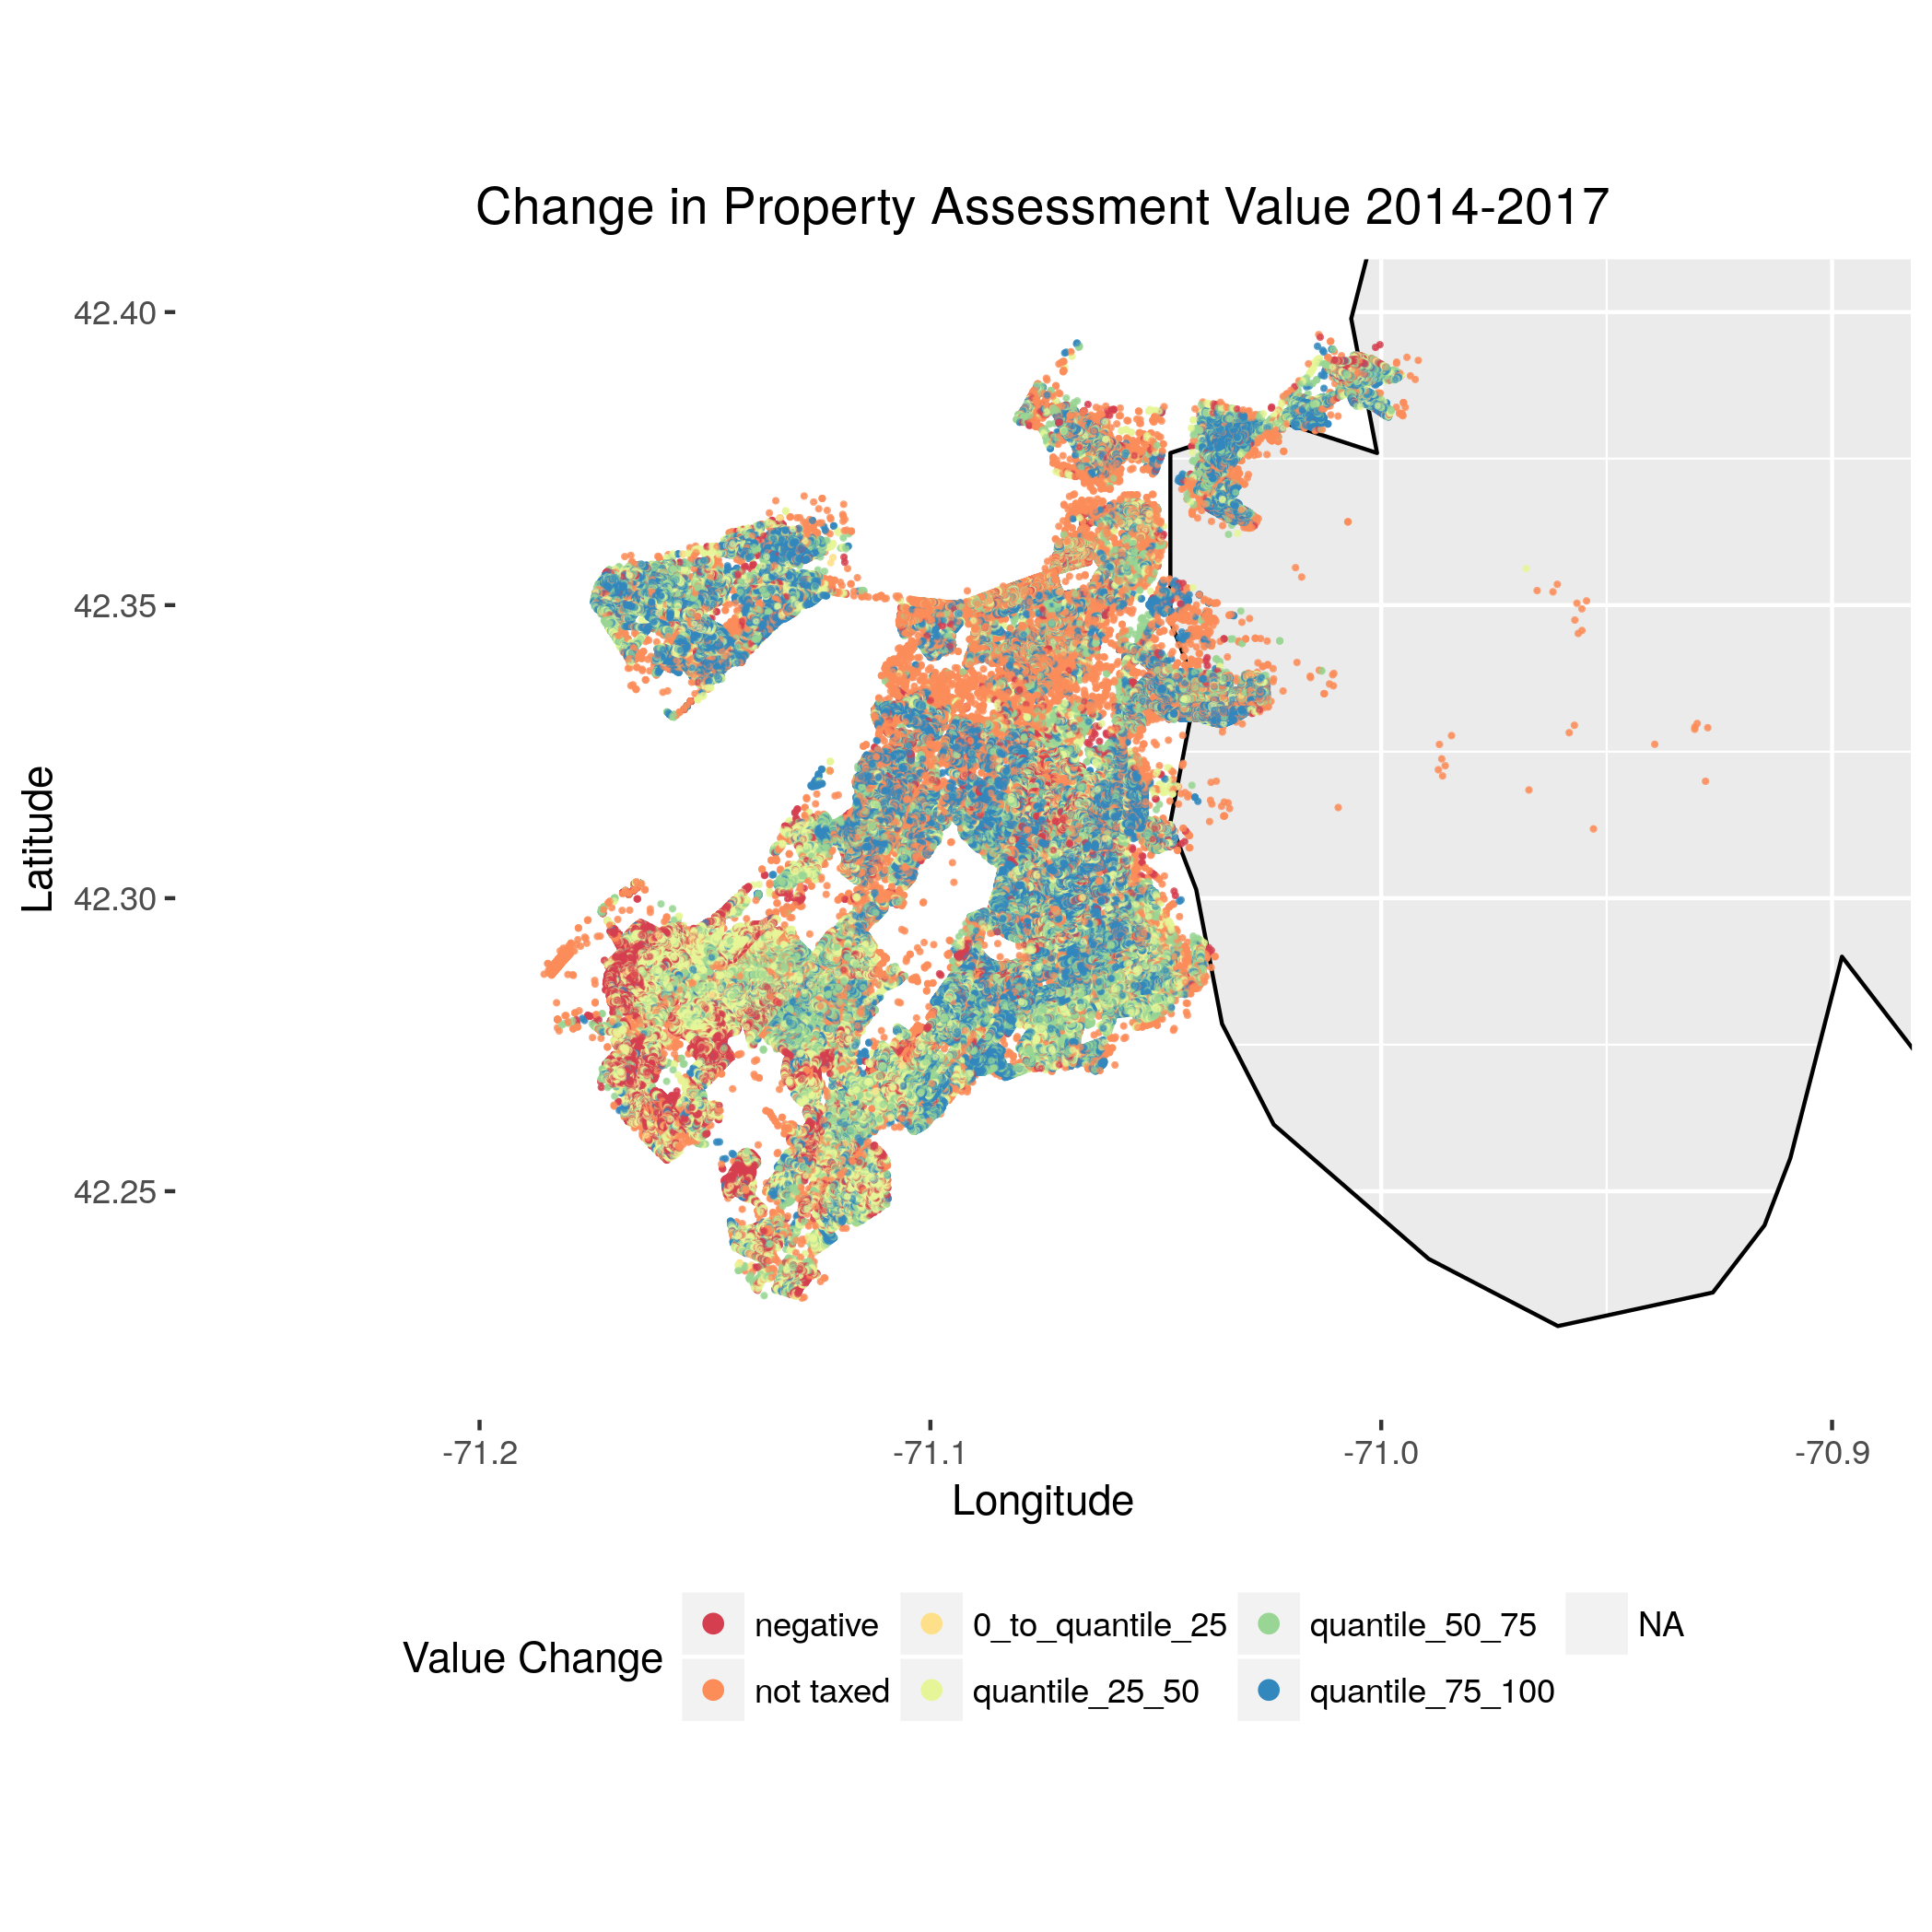
\includegraphics[scale=0.75]{property_delta2014-2017}


\bibliography{references} 
\bibliographystyle{ieeetr}

\end{document}
